

\begin{mydef}
	\iftoggle{eleve}{%
		Deux figures sont \hrulefill
		
		\vspace*{0.2cm}
		\hrulefill
		
		\vspace*{0.2cm}
		\hrulefill
		
		\vspace*{0.2cm}
		\hrulefill
	}{%

	Deux figures sont \kw{symétriques par rapport à un point $O$} si elles se superposent lorsqu'on effectue un demi-tour autour du point $O$. Le point $O$ est appelé \kw{centre de symétrie}.
}	
\end{mydef}

\begin{myex}
	\begin{center}
		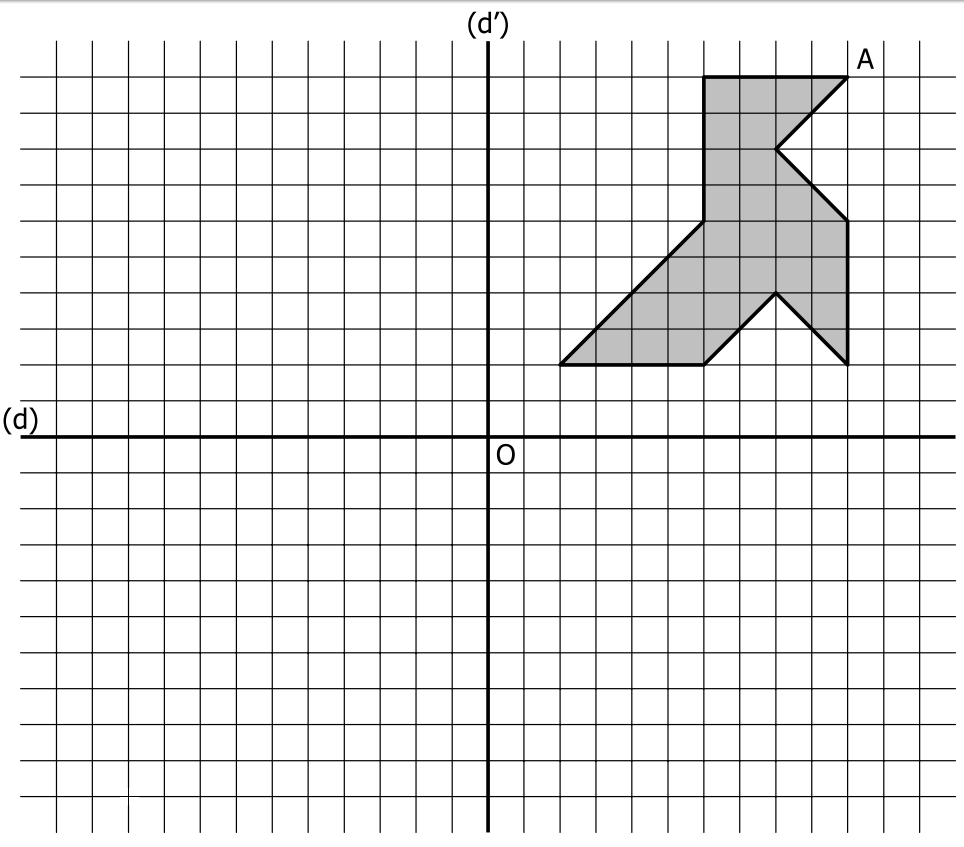
\includegraphics[scale=.5]{fig2}
	\end{center}
\end{myex}

\begin{mydef}
	\iftoggle{eleve}{%
		Dire que deux points $M$ et $M'$ \hrulefill
		
		\vspace*{0.2cm}
		\hrulefill
		
		\vspace*{0.2cm}
		\hrulefill
		

	}{%
	Dire que deux points $M$ et $M'$ sont symétriques par rapport à un point $O$ signifie que le point $O$ est le milieu du segment $[MM']$.
	}
\end{mydef}

\begin{myex}
	\begin{center}
		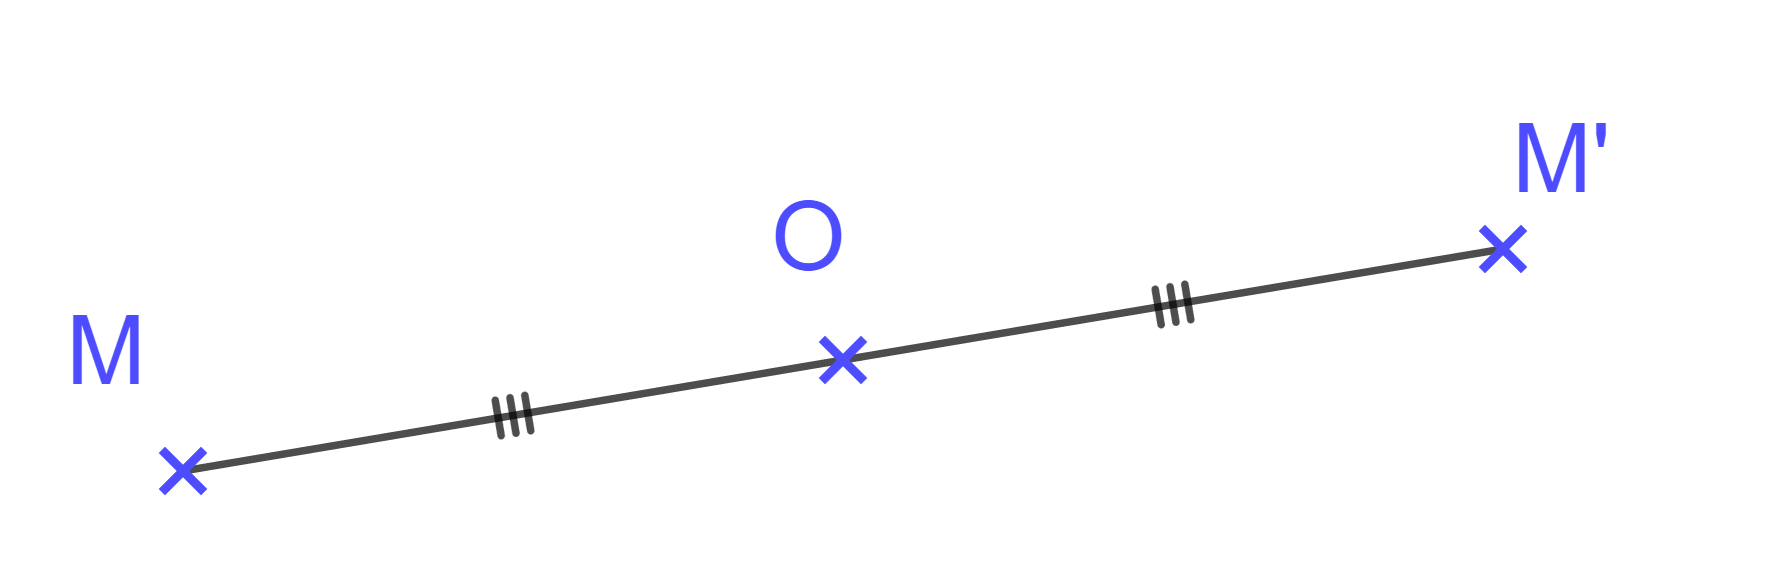
\includegraphics[scale=.25]{fig3}
	\end{center}
\end{myex}

\begin{myremarque}
	\iftoggle{eleve}{%
		Pour construire le \hrulefill
		
		\vspace*{0.2cm}
		\hrulefill
		
		\vspace*{0.2cm}
		\hrulefill
		
		
	}{%
		Pour construire le symétrique du point $M$, on reporte au compas la longueur $OM$ sur la demi-droite $[MO)$.
	}
\end{myremarque}